% Created 2024-11-07 Thu 14:40
% Intended LaTeX compiler: xelatex

\documentclass[10pt]{beamer}

% fonts
\usepackage{ctex}
\usepackage{fontspec}
\setmainfont{Times New Roman}
\setmonofont{Inconsolata}
\setsansfont{Times New Roman}
\setCJKmainfont{STSong}
\setCJKsansfont{SimSong}
\setCJKmonofont{LXGW WenKai Mono}

\usepackage{amsfonts}
\usepackage{amsthm}
\usepackage{bm}
\usepackage{siunitx}
\usepackage{xcolor}

\usepackage{mathrsfs}
% commands
\newcommand{\mr}[1]{\mathrm{#1}}
\newcommand{\mb}[1]{\mathbf{#1}}
\newcommand{\mc}[1]{\mathcal{#1}}
\newcommand{\ms}[1]{\mathscr{#1}}

\usepackage{graphicx}
\usepackage{longtable}
\usepackage{wrapfig}
\usepackage{rotating}
\usepackage[normalem]{ulem}
\usepackage{amsmath}
\usepackage{amssymb}
\usepackage{capt-of}
\usepackage{hyperref}
\usepackage{etoolbox}
\usepackage{pgfopts}
\usepackage{booktabs}
\usepackage[scale=2]{ccicons}
\usetheme[block=fill, progressbar=frametitle]{metropolis}
\useoutertheme{infolines} % 采用 infoline
\useinnertheme{default}
\usecolortheme{custom} % 使用 custom 颜色主题
\setbeamertemplate{blocks}[rounded][shadow=false]
\setbeamertemplate{items}[circle] % circle item symbol
\setbeamertemplate{sections/subsections in toc}[ball] % ball section symbol
\setbeamertemplate{headline}[default] % 不使用 infoline 的 headline
%\setbeamertemplate{footline}[default] % 使用 infoline 的 footline
\setbeamertemplate{frame numbering}[none]
\setbeamertemplate{bibliography item}[text] % 使用 text 的 references 形式
%\setbeamerfont{footnote}{\tiny} % 可选择 tiny footnote
\usetheme{default}
\author{王亚朋 \quad 报告人: 朱宇涛}
\date{2024年 11 月 7日}
\title{Michel电子能谱测量}
\subtitle{宇宙线粒子探测与物理实验}

\hypersetup{
pdfauthor={王亚朋 \quad 报告人: 朱宇涛},
pdftitle={Michel电子能谱测量},
pdfkeywords={},
pdfsubject={},
pdfcreator={Emacs 29.1 (Org mode 9.6.6)},
pdflang={Cn},
colorlinks=true,
linkcolor=black
}
\begin{document}

\maketitle
\begin{frame}[label={sec:org39e6fb4}]{目录}
\tableofcontents
\end{frame}

\section{实验内容}
\label{sec:org61d0955}
\begin{frame}[label={sec:orgf1f30f5}]{实验内容}
\begin{enumerate}
\item 在左右两端电压 1500V 且甄别阈 25mV 的实验条件下, 重新测量了衰减长度和能量刻度.
\item 在相同实验条件下测量了 Michel 电子能谱.
\end{enumerate}
\end{frame}
\section{实验结果}
\label{sec:org2018d95}
\begin{frame}[label={sec:org7acc9f6}]{衰减长度}
\begin{figure}[htbp]
\centering
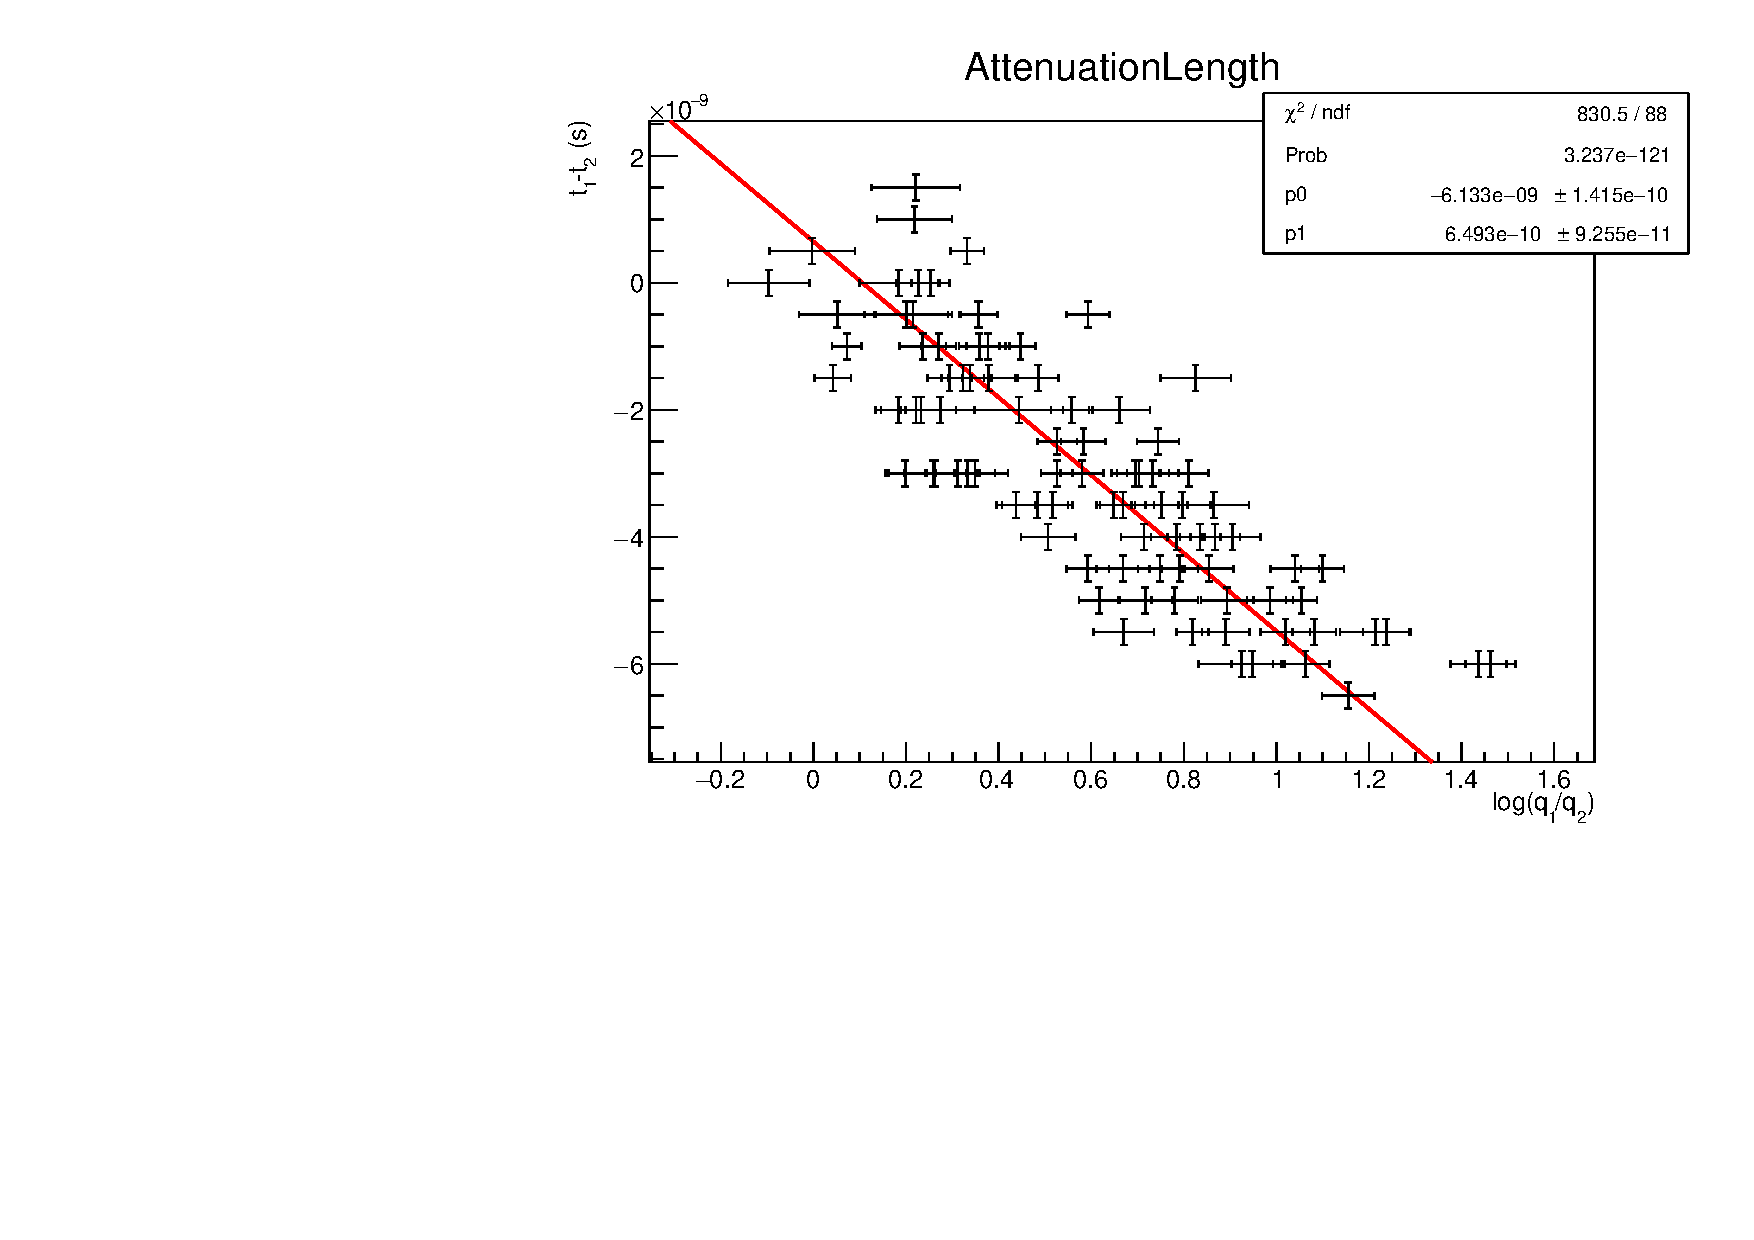
\includegraphics[width=0.5\textwidth]{../../DetectorPerform/AttenuationLength/figs/ReReAttenuationLength.pdf}
\caption{衰减长度}
\end{figure}

衰减长度和相关系数:
\begin{align*}
L_0 &= 1.162 \pm \qty{0.027}{m} \\
R^2 &= 0.684.
\end{align*}
\end{frame}

\begin{frame}[label={sec:org527b8a9}]{能量刻度}
由于测量 Michel 电子能谱时重新调节左右两端电压均为 1500V 且甄别阈为 25mV, 故需要重新进行能量刻度.

挑选 100 个 \(\mu\) 信号进行刻度得到:

\begin{columns}
\begin{column}{0.5\columnwidth}
\begin{figure}[htbp]
\centering
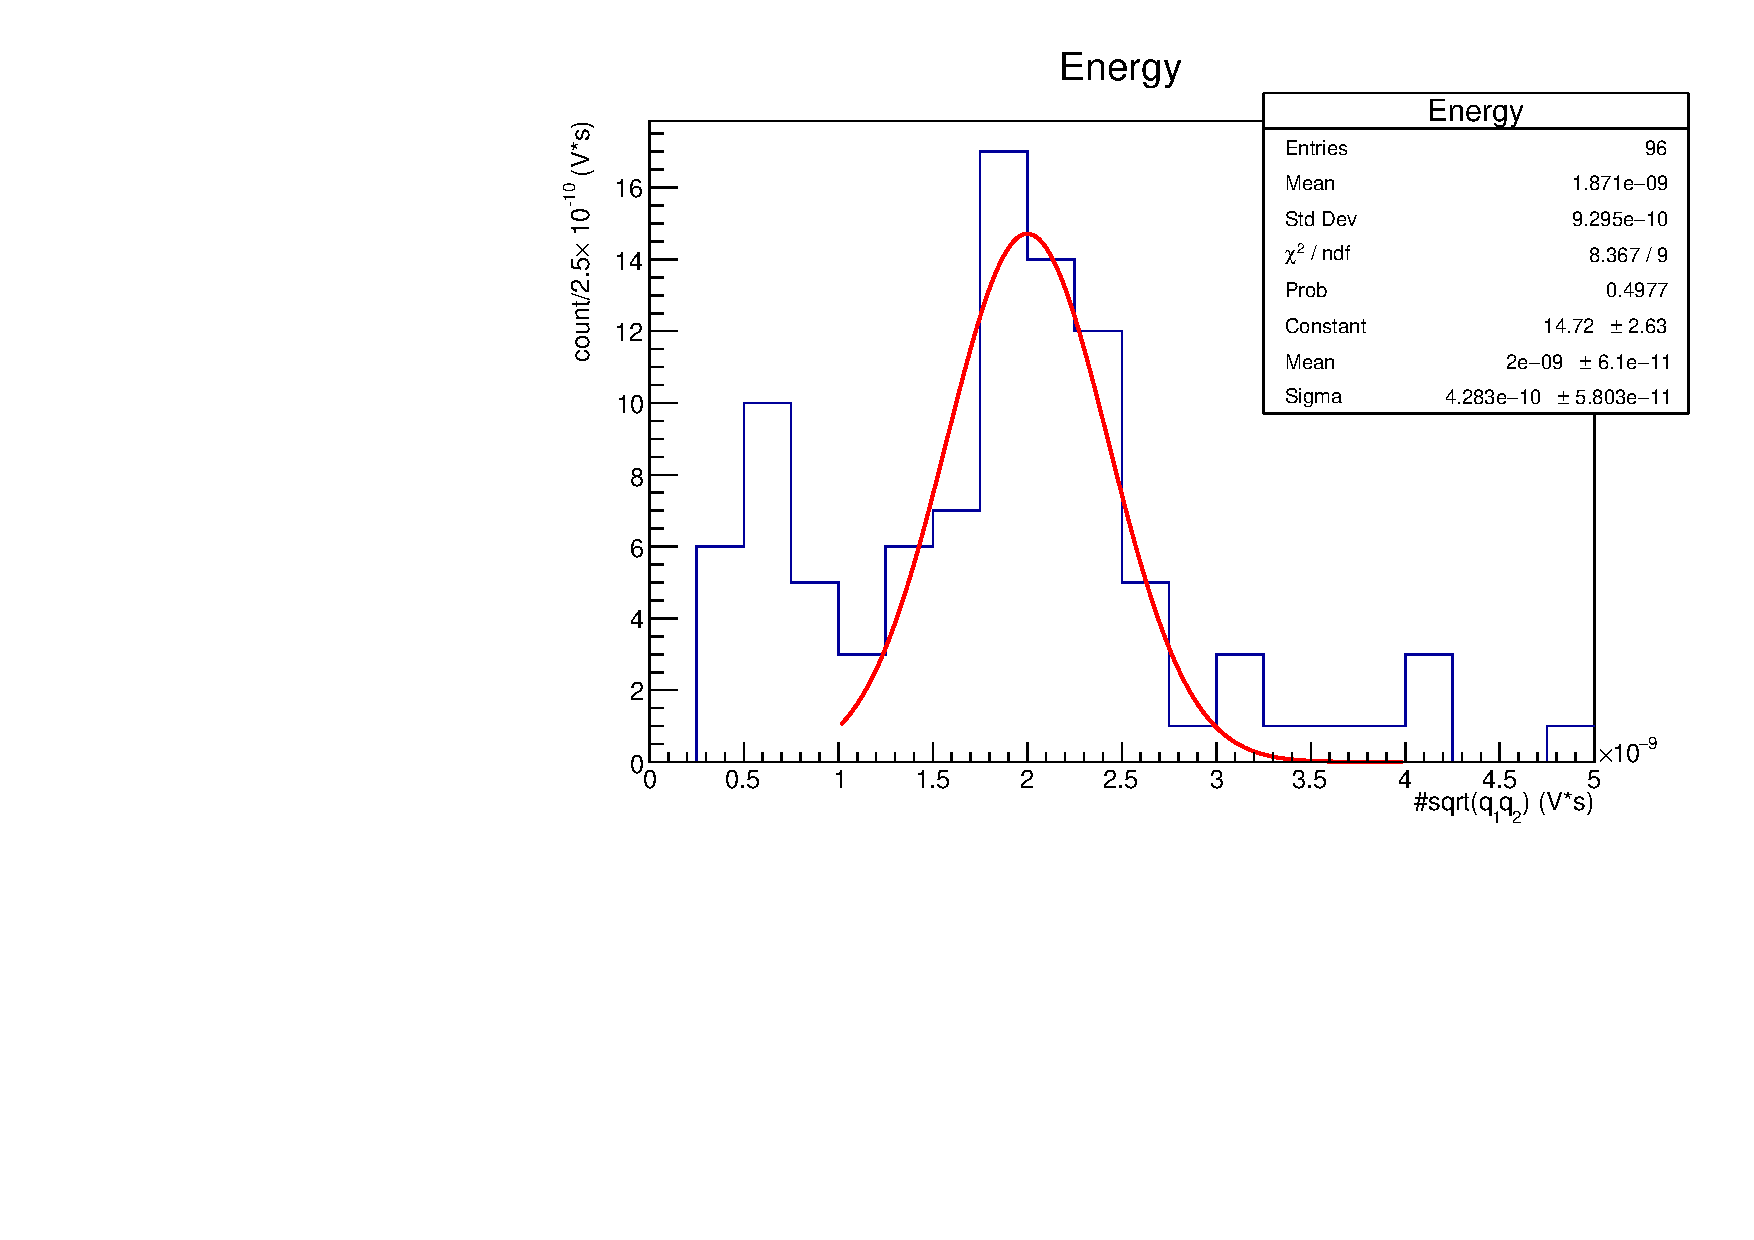
\includegraphics[width=1.0\textwidth]{../../DetectorPerform/ECali/reqqdist.pdf}
\caption{能量刻度}
\end{figure}
\end{column}

\begin{column}{0.5\columnwidth}
\begin{itemize}
\item 刻度系数为 \num{5.017e9}.
\item 能量分辨率为
\begin{equation*}
\frac{2.35\sigma}{\mu} = \frac{\num{4.305e-10}}{\num{1.987e-09}} = 21.7\%.
\end{equation*}
\end{itemize}
\end{column}
\end{columns}
\end{frame}
\begin{frame}[label={sec:orgffd5cf0}]{Michel 电子能谱}
\begin{itemize}
\item 理论上, Michel 电子能谱应当服从 Beta 分布\footnote{\url{https://dspace.mit.edu/bitstream/handle/1721.1/121063/1704.02927.pdf}}.
\item 实验得到的 Michel 左侧部分不符合, 可能与能量刻度左侧的峰对应.
\end{itemize}

\begin{columns}
\begin{column}{0.5\columnwidth}
\begin{figure}[htbp]
\centering
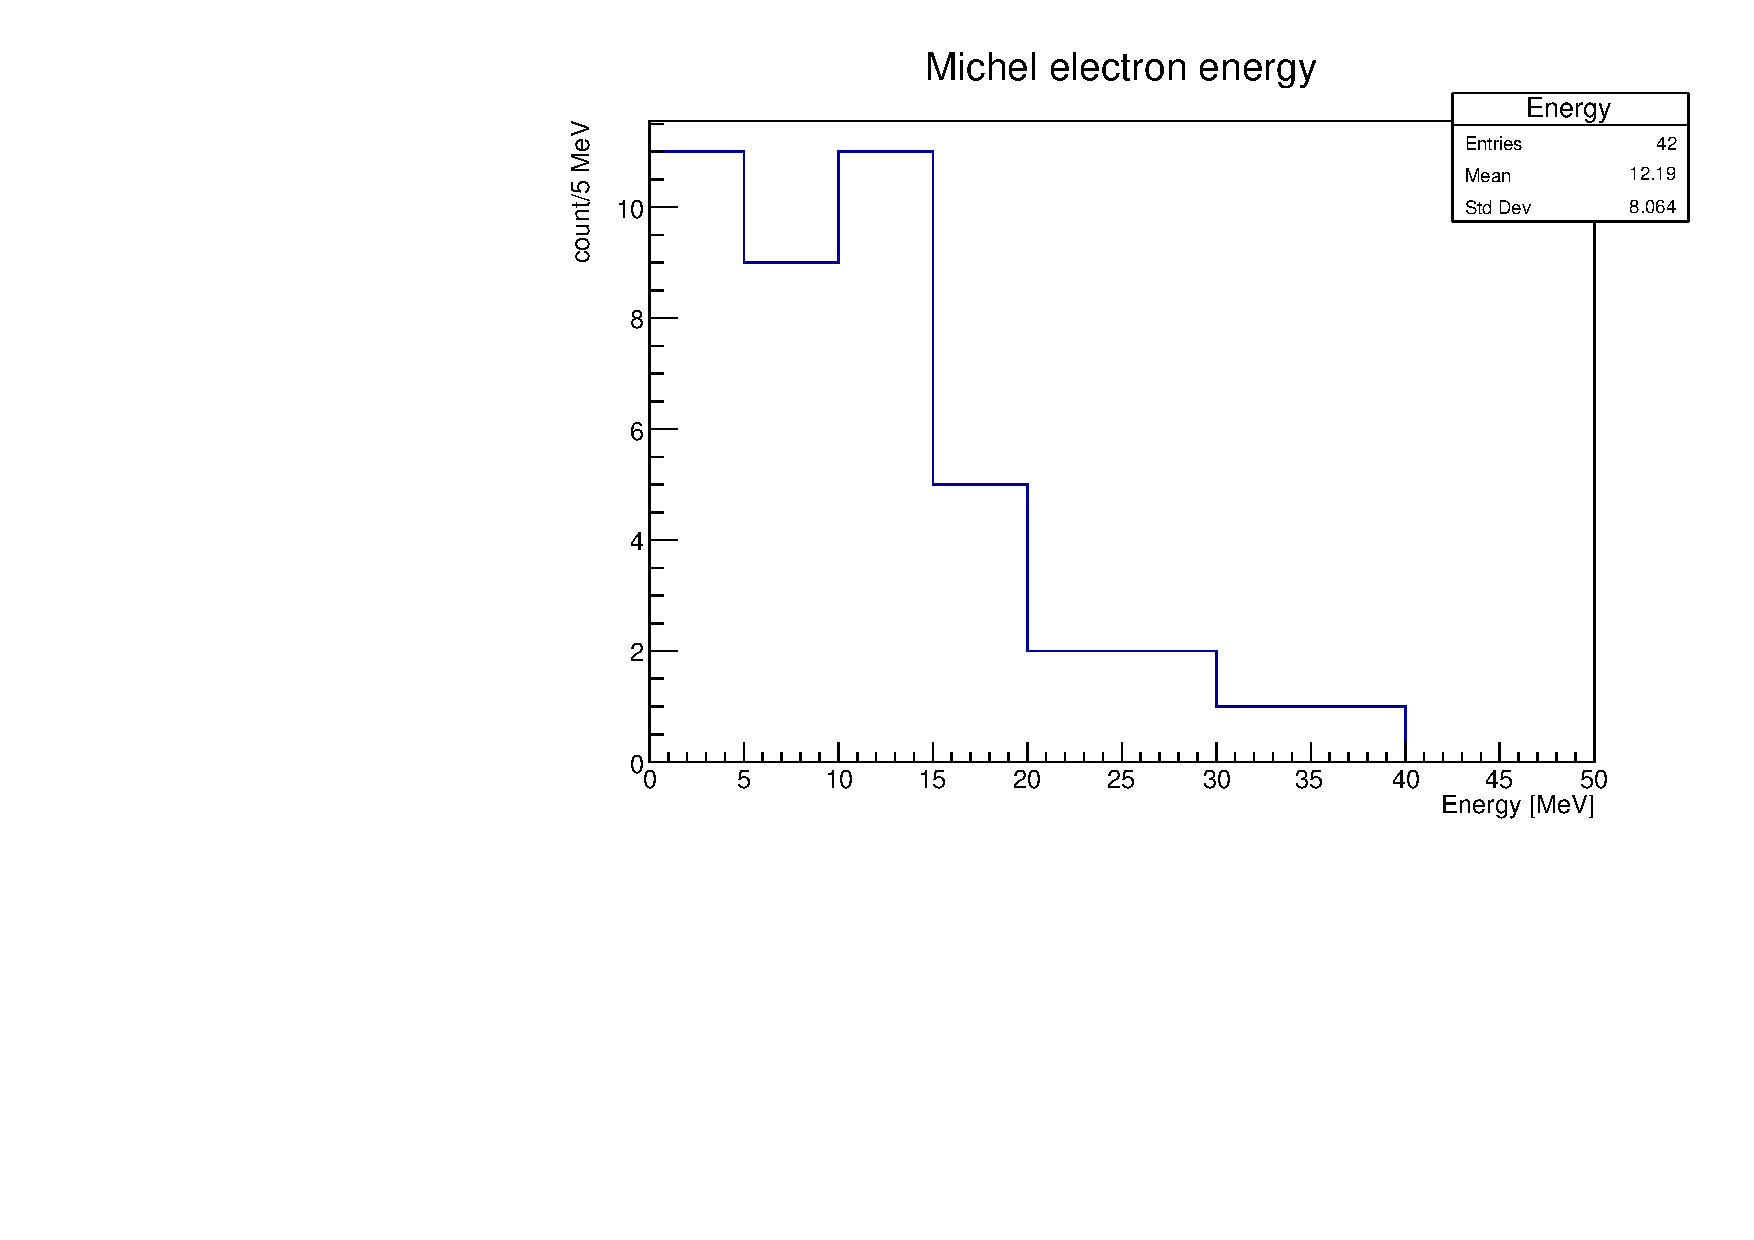
\includegraphics[width=0.9\textwidth]{../../mu/michel/michel.pdf}
\caption{Michel 电子能谱}
\end{figure}
\end{column}

\begin{column}{0.5\columnwidth}
\begin{figure}[htbp]
\centering
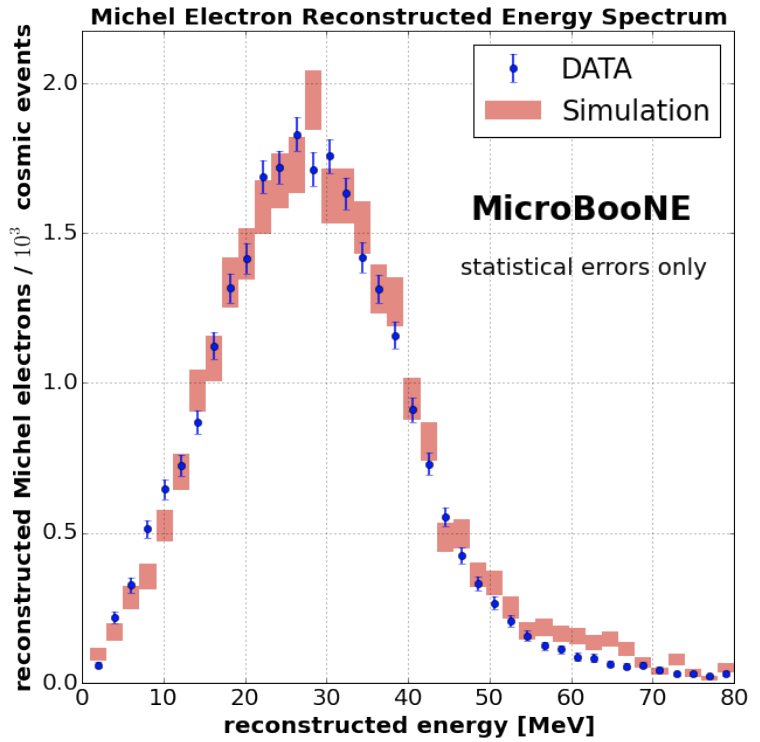
\includegraphics[width=0.8\textwidth]{../../img/michelPaper.pdf}
\caption{Michel 电子能谱(MicroBooNE)}
\end{figure}
\end{column}
\end{columns}
\end{frame}
\end{document}